% Created 2017-04-04 Tue 09:58
% Intended LaTeX compiler: pdflatex
\documentclass[a4paper,11pt]{article}
\usepackage[utf8]{inputenc}
\usepackage[T1]{fontenc}
\usepackage{graphicx}
\usepackage{grffile}
\usepackage{longtable}
\usepackage{wrapfig}
\usepackage{rotating}
\usepackage[normalem]{ulem}
\usepackage{amsmath}
\usepackage{textcomp}
\usepackage{amssymb}
\usepackage{capt-of}
\usepackage{hyperref}
\usepackage[margin=1.2in]{geometry}
\usepackage{setspace}
\onehalfspacing
\usepackage{parskip}
\usepackage{amsthm}
\usepackage{amsmath}
\usepackage{mathtools}
\usepackage{hyperref}
\usepackage{graphicx}
\usepackage{tabularx}
\usepackage{booktabs}
\usepackage{color}
\usepackage{caption}
\usepackage{subcaption}
\hypersetup{colorlinks,citecolor=black,filecolor=black,linkcolor=black,urlcolor=black}
\newtheorem{mydef}{Definition}
\newtheorem{mythm}{Theorem}
\newcommand{\dx}{\mathrm{d}}
\newcommand{\var}{\mathrm{Var}}
\newcommand{\cov}{\mathrm{Cov}}
\newcommand{\corr}{\mathrm{Corr}}
\newcommand{\pr}{\mathrm{Pr}}
\newcommand{\rarrowd}[1]{\xrightarrow{\text{ \textit #1 }}}
\renewcommand\chaptername{Lecture}
\DeclareMathOperator*{\plim}{plim}
\newcommand{\plimn}{\plim_{n \rightarrow \infty}}
\setcounter{secnumdepth}{2}
\author{Zheng Tian}
\date{}
\title{Lecture 8: Linear Regression with Multiple Regressors}
\hypersetup{
 pdfauthor={Zheng Tian},
 pdftitle={Lecture 8: Linear Regression with Multiple Regressors},
 pdfkeywords={},
 pdfsubject={},
 pdfcreator={Emacs 25.1.1 (Org mode 9.0.3)}, 
 pdflang={English}}
\begin{document}

\maketitle

\section{Introduction}
\label{sec:orga1ac16b}
\subsection{Overview}
\label{sec:orgc26a6a7}
This lecture extends the simple regression model to the multiple
regression model. Many aspects of multiple regression parallel those
of regression with a single regressor. The coefficients of the
multiple regression model can be estimated using the OLS estimation
method. The algebraic and statistical properties of the OLS estimators
of the multiple regression are also similar to those of the simple
regression. However, there are some new concepts, such as the
omitted variable bias and multicollinearity, to deepen our
understanding of the OLS estimation.

\subsection{Learning goals}
\label{sec:org63af751}
\begin{itemize}
\item Be able to set up a multiple regression model with matrix notation.
\item Understand the meaning of holding other things constant.
\item Estimate the multiple regression model with the OLS estimation.
\item Understand the Frisch-Waugh-Lovell theorem.
\item Capable of detecting the omitted variable bias and
multicollinearity.
\end{itemize}

\subsection{Readings}
\label{sec:org2b822a3}
\begin{itemize}
\item \emph{Introduction to Econometrics} by Stock and Watson. Read thoroughly
Chapter 6 and Sections 18.1 and 18.2
\item \emph{Introductory Econometrics: a Modern Approach} by
Wooldridge. Chapter 3.
\end{itemize}
\section{The Multiple Regression Model}
\label{sec:org7d2d480}
\subsection{The problem of a simple linear regression}
\label{sec:org8f872c4}
In the last two lectures, we use a simple linear regression model to
examine the effect of class sizes on test scores in the California
elementary school districts. The simple linear regression model with
only one regressor is
\begin{equation*}
TestScore = \beta_0 + \beta_1 \times STR + OtherFactors
\end{equation*}

\subsubsection*{What are your intuitive challenge against this model?}
\label{sec:org6f0d29e}
\begin{itemize}
\item It ignores too many other important factors that are presumably
included in \emph{OtherFactors}, which is the error term, \(u_i\), in the
regression model.
\begin{itemize}
\item What are possible other important factors?
\begin{description}
\item[{School characteristics}] teachers' quality, school buildings, equipment
\item[{Student characteristics}] family economic conditions, individual
ability
\end{description}
\end{itemize}
\end{itemize}

\subsubsection*{Percentage of English learners as an example}
\label{sec:org9dcbb4f}

The percentage of English learners in a school district could be an
relevant and important determinant of test scores, which is omitted
in the simple regression model.

\begin{itemize}
\item How can it affect the estimate of the effect of student-teacher ratios on test score?
\label{sec:orgd19aaa0}

\begin{itemize}
\item The districts with high percentages of English learners tend to have
large student-teacher ratios. That is, these two variables are
correlated with the correlation coefficient being 0.17.
\item The higher percentage of English learners a district has, the lower
test scores students there will make.
\item In the simple regression model, the estimated negative coefficient on
student-teacher ratios on test scores could include not only the
negative influence from class sizes but also that from the
percentage of English learners.
\item In the terminology of statistics, the magnitude of the coefficient
on student-teacher ratio is \textbf{overestimated}.
\item Generally, we commit an \textbf{omitted variable bias} by setting up a simple
regression model. We will explore the omitted variable bias in the
last section in this lecture.
\end{itemize}

\item Solutions to the omitted variable bias
\label{sec:org79495ea}

Include the percentage of English learners in the regression model.
\[ TestScore_i = \beta_0 + \beta_1 STR_i + \beta_2 PctEL_i + OtherFactors_i \]
which is a multiple regression model. In fact, we can include other independent
variables in the multiple regression model.
\end{itemize}

\subsection{The form of a multiple regression model}
\label{sec:org436f0f3}
The general form of a \textbf{multiple regression model} is
\begin{equation}
\label{eq:multi-regress-1}
Y_i = \beta_0 + \beta_1 X_{1i} + \beta_2 X_{2i} + \cdots + \beta_k X_{ki} + u_i,\; i = 1, \ldots, n
\end{equation}
where
\begin{itemize}
\item \(Y_i\) is the i\(^{\text{th}}\) observation on the dependent variable; \(X_{1i},
  X_{2i}, \ldots, X_{ki}\) are the i\(^{\text{th}}\) observation on each of the
\(k\) regressors; and \(u_i\) is the error term associated with the
i\(^{\text{th}}\) observation.
\item The \textbf{population regression line} (or \textbf{population regression
function}) is the relationship that holds between \(Y\) and \(X\) on
average in the population
\begin{equation*}
E(Y_i | X_{1i} = x_{1}, \ldots, X_{ki} = x_k) = \beta_0 + \beta_1 x_1 + \cdots + \beta_k x_k
\end{equation*}
\item \(\beta_1, \ldots, \beta_k\) are the coefficients on the corresponding
\(X_i,\, i = 1, \ldots, k\). \(\beta_0\) is the intercept, which can
also be thought of the coefficient on a regressor \(X_{0i}\) that equals
1 for all observations.
\begin{itemize}
\item Including \(X_{0i}\), there are \(k+1\) regressors in the multiple
regression model.
\item The linear regression model with a single regressor is in fact a
multiple regression model with two regressors, 1 and \(X\).
\end{itemize}
\item \(u_i\) is the error term. It can be assumed to be \textbf{homoskedastic}.
That is, \(\var(u_i | X_{1i}, \ldots, X_{ki}) = \sigma^2_u\), which is
a constant independent of the value of \(X_{1i}, \ldots,
  X_{ki}\). Otherwise, it can be assumed to be \textbf{heteroskedastic}.
\end{itemize}

\subsection{The interpretation of \(\beta_i\)}
\label{sec:org771fdfa}
\subsubsection*{Holding other things constant}
\label{sec:orgde7ed4b}
We can suppress the subscript \(i\) in Equation (\ref{eq:multi-regress-1})
so that we can re-write it as

\begin{equation}
\label{eq:multi-regress-1a}
Y = \beta_0 + \beta_1 X_1 + \cdots + \beta_k X_k + u
\end{equation}

In the multiple regression model in Equation
(\ref{eq:multi-regress-1a}), the coefficient \(\beta_i\) on the regressor
\(X_i\) for \(i=1, \ldots, k\) measures the effect on \(Y\) of a unit change
in \(X_i\), \textbf{holding other \(X\) constant} or \textbf{controlling for other
\(X\)}.

The phrase of \textbf{holding other things constant} (or \textbf{ceteris paribus} in
Latin) is important in economics. To disentangle the particular causal
effect of one explanatory variable \(X\) on \(Y\) from all other
confounding factors, we must hold these other factors constant so that
it is meaningful to compare the values of \(Y\) before and after a
change in \(X\) happens.

Suppose we have two regressors \(X_1\) and \(X_2\) and we are interested
in the effect of \(X_1\) on \(Y\). We can let \(X_1\) change by \(\Delta X\)
and holding \(X_2\) constant. Then, the new value of \(Y\) is
\[ Y + \Delta Y = \beta_0 + \beta_1 (X_1 + \Delta X_1) + \beta_2 X_2  \]
By subtracting \(Y = \beta_0 + \beta_1 X_1 + \beta_2 X_2\), we have
\(\Delta Y = \beta_1 \Delta X_1\). That is
\[ \beta_1 = \frac{\Delta Y}{\Delta X} \text{ holding } X_2 \text{ constant} \]

\subsubsection*{Partial effect}
\label{sec:orge9349cc}
If \(Y\) and \(X_i\) for \(i = 1, \ldots, k\) are continuous and
differentiated variables, from Equation (\ref{eq:multi-regress-1a}),
we know that \(\beta_i\) is as simply as the partial derivative of \(Y\) with
respect to \(X_i\). That is \[\beta_i = \frac{\partial Y}{\partial
X_i}\] By the definition of a partial derivative, \(\beta_i\) is just
the effect of a marginal change in X on \(Y\) holding other \(X\)
constant.

\subsection{The matrix notation of a multiple regression model}
\label{sec:org9237f5d}
\subsubsection*{Consider the matrix notation as a way to organize data}
\label{sec:orgec2fbb6}
When we save the data set of California school districts in Excel, it
is saved in a spreadsheet like the following,

\begin{figure}[htbp]
\centering
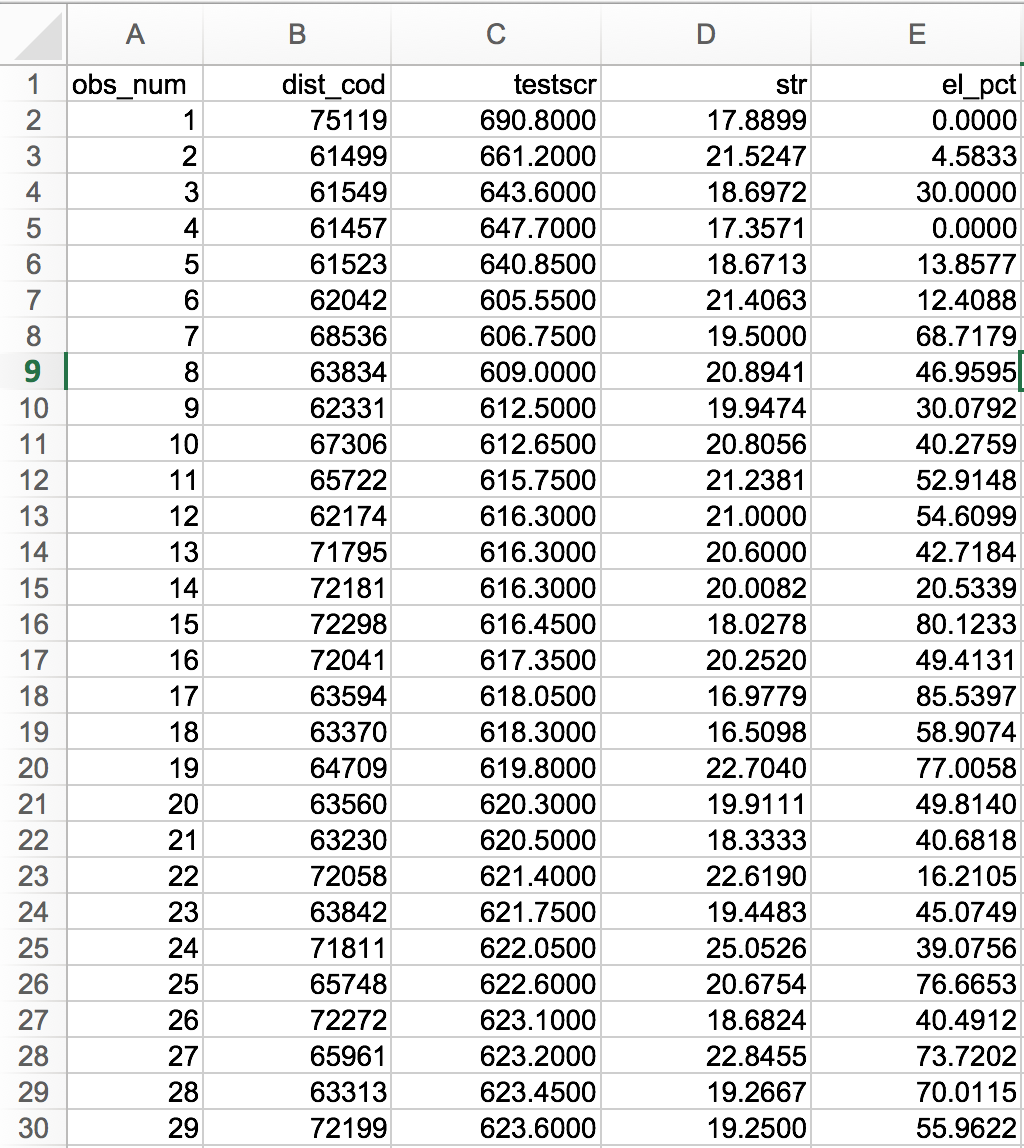
\includegraphics[width=0.7\textwidth]{img/data_snapshot.png}
\caption{\label{fig:org7ffc0db}
The California data set in Excel}
\end{figure}

Each row represents an observation of all variables pertaining to a
school district, and each column represents a variable with all
observations. This format of data display can be concisely denoted
using vectors and a matrix.

Let us first define the following vectors and matrices:
\begin{equation*}
\mathbf{Y} =
\begin{pmatrix}
Y_1 \\
Y_2 \\
\vdots \\
Y_n
\end{pmatrix},\,
\mathbf{X} =
\begin{pmatrix}
1 & X_{11} & \cdots & X_{k1} \\
1 & X_{12} & \cdots & X_{k2} \\
\vdots & \vdots & \ddots & \vdots \\
1 & X_{1n} & \cdots & X_{kn}
\end{pmatrix}
=
\begin{pmatrix}
\mathbf{X}^{\prime}_1 \\
\mathbf{X}^{\prime}_2 \\
\vdots \\
\mathbf{X}^{\prime}_n
\end{pmatrix},\,
\mathbf{U} =
\begin{pmatrix}
u_1 \\
u_2 \\
\vdots \\
u_n
\end{pmatrix},\,
\boldsymbol{\beta} =
\begin{pmatrix}
\beta_0 \\
\beta_1 \\
\vdots \\
\beta_k
\end{pmatrix}
\end{equation*}

\begin{itemize}
\item \(\mathbf{Y}\) is an \(n \times 1\) vector of \(n\) observations on the
dependent variable.
\item \(\mathbf{X}\) is an \(n \times (k+1)\) matrix of \(n\) observations on
\(k + 1\) regressors which include the intercept term as a regressor of
1's.
\item \(\mathbf{X}_i\) is a \((k+1) \times 1\) vector of the i\(^{\text{th}}\)
observation on all \((k+1)\) regressors. Thus,
\(\mathbf{X}^{\prime}_i\) denotes the i\(^{\text{th}}\) row in \(\mathbf{X}\).
\item \(\boldsymbol{\beta}\) is a \((k+1) \times 1\) vector of the \((k+1)\)
regression coefficients.
\item \(\mathbf{U}\) is an \(n \times 1\) vector of the \(n\) error terms.
\end{itemize}

\subsubsection*{Write a multiple regression model with matrix notation}
\label{sec:org8f35142}
\begin{itemize}
\item The multiple regression model for one observation
\label{sec:org8a2f15a}

The multiple regression model in Equation (\ref{eq:multi-regress-1})
for the i\(^{\text{th}}\) observation can be written as
\begin{equation}
\label{eq:multi-regress-mi}
Y_i = \mathbf{X}^{\prime}_i \boldsymbol{\beta} + u_i,\; i = 1, \ldots, n
\end{equation}

\item The multiple regression model for all observations
\label{sec:orgfdb6a2c}

Stacking all \(n\) observations in Equation (\ref{eq:multi-regress-mi})
yields the multiple regression model in matrix form:
\begin{equation}
\label{eq:multi-regress-m}
\mathbf{Y} = \mathbf{X} \boldsymbol{\beta} + \mathbf{U}
\end{equation}

\(\mathbf{X}\) can also be written in terms of column vectors as
\[
\mathbf{X} = [\boldsymbol{X}_0, \boldsymbol{X}_1, \ldots, \boldsymbol{X}_k ]
\]
where \(\boldsymbol{X}_i = [X_{i1}, X_{i2}, \ldots, X_{in}]^{\prime}\) is a
\(n \times 1\) vector of \(n\) observations of the k\(^{\text{th}}\)
regressor. \(\boldsymbol{X}_0\) is a vector of 1s. That is,
\(\boldsymbol{X}_0 = [1, 1, \ldots, 1]^{\prime}\). More often, we use
\(\boldsymbol{\iota}\) to denote such a vector of 1s. \footnote{\(\boldsymbol{\iota}\) has the following properties:
(1) \(\boldsymbol{\iota}^{\prime} \mathbf{x} = \sum_{i=1}^n x_i\) for an
  \(n \times 1\) vector \(\mathbf{x}\), (2) \(\boldsymbol{\iota}^{\prime}
\boldsymbol{\iota} = n\) and \(\left(\boldsymbol{\iota}^{\prime}
\boldsymbol{\iota} \right)^{-1} = 1/n\), (3)
\(\boldsymbol{\iota}^{\prime} \left(
\boldsymbol{\iota}^{\prime}\boldsymbol{\iota} \right)^{-1} \mathbf{x}
= \bar{x}\), and (4) \(\boldsymbol{\iota}^{\prime} \mathbf{X} \boldsymbol{\iota} =
  \sum_{i=1}^n \sum_{j=1}^n x_{ij}\) for an \(n \times n\) matrix \(\mathbf{X}\).}

Thus, Equation (\ref{eq:multi-regress-m}) can be re-written as
\begin{equation}
\label{eq:multi-regress-m2}
\mathbf{Y} = \beta_0\boldsymbol{\iota} + \beta_1\boldsymbol{X}_1 + \cdots + \beta_k\boldsymbol{X}_k + \mathbf{U}
\end{equation}
\end{itemize}

\section{The OLS Estimator in Multiple Regression}
\label{sec:orge3bca9a}
\subsection{The OLS estimator}
\label{sec:org6cbdab2}
\subsubsection*{The minimization problem}
\label{sec:org0ea01f6}
The idea of the ordinary least squares estimation for a multiple
regression model is exactly the same as for a simple regression
model. The OLS estimators of the multiple regression model are obtained by
minimizing the sum of the squared prediction mistakes.

Let \(\mathbf{b} = [b_0, b_1, \ldots, b_k]^{\prime}\) be some estimators of
\(\boldsymbol{\beta} = [\beta_0, \beta_1, \ldots,
\beta_k]^{\prime}\). The predicted \(Y_i\) can be obtained by
\[ \hat{Y}_i = b_0 + b_1 X_{1i} + \cdots + b_k X_{ki} = \mathbf{X}^{\prime}_i
\mathbf{b},\, i = 1, \ldots, n \]
or
\[ \hat{\mathbf{Y}} = \mathbf{Xb} \]

The prediction mistakes with \(\mathbf{b}\), or called the residuals, are
\[ \hat{u}_i = Y_i - b_0 - b_1 X_{1i} - \cdots - b_k X_{ki} = Y_i -
\mathbf{X}^{\prime}_i \mathbf{b} \]
or in vector notation, the residual vector is
\[ \hat{\mathbf{u}} = \mathbf{Y} - \mathbf{Xb} \]

Then the sum of the squared prediction mistakes (residuals) is
\begin{align*}
S(\mathbf{b}) & = S(b_0, b_1, \ldots, b_k) = \sum_{i=1}^n (Y_i - b_0 - b_1 X_{1i} - \cdots - b_k X_{ki})^2 \\
& = \sum_{i=1}^n (Y_i - \mathbf{X}^{\prime}_i \mathbf{b})^2 = (\mathbf{Y} -
\mathbf{Xb})^{\prime}(\mathbf{Y}-\mathbf{Xb}) \\
& = \hat{\mathbf{u}}^{\prime} \hat{\mathbf{u}} = \sum_{i=1}^n \hat{u}_i^2
\end{align*}

The OLS estimator is the solution to the following minimization problem:
\begin{equation}
\label{eq:ols-multi-regress}
\operatorname*{min}_{\mathbf{b}}\: S(\mathbf{b}) = \hat{\mathbf{u}}^{\prime} \hat{\mathbf{u}}
\end{equation}

\subsubsection*{The OLS estimator of \(\boldsymbol{\beta}\) as a solution to the minimization problem}
\label{sec:org9034f3a}
The formula for the OLS estimator is obtained by taking the derivative
of the sum of squared prediction mistakes, \(S(b_0, b_1, \ldots, b_k)\), with respect to each coefficient,
setting these derivatives to zero, and solving for the estimator
\(\hat{\boldsymbol{\beta}}\).

The derivative of \(S(b_0, \ldots, b_k)\) with respect to \(b_j\) is
\begin{gather*}
\label{eq:ols-wrt-bj}
\frac{\partial }{\partial b_j} \sum_{i=1}^n \left(Y_i - b_0 - b_1 X_{1i} - \cdots - b_k X_{ki} \right)^2 = \\
-2 \sum_{i=1}^n X_{ji} \left(Y_i - b_0 - b_1 X_{1i} - \cdots - b_k X_{ki} \right) = 0
\end{gather*}
There are \(k+1\) such equations for \(j=0, \ldots, k\). Solving this
system of equations, we obtain the OLS estimator
\(\hat{\boldsymbol{\beta}} = (b_0, \ldots, b_k)^{\prime}\).

Using matrix notation, the formula for the OLS estimator
\(\boldsymbol{\hat{\beta}}\) is
\begin{equation}
\label{eq:betahat-mult}
\boldsymbol{\hat{\beta}} = (\mathbf{X}^{\prime} \mathbf{X})^{-1} \mathbf{X}^{\prime} \mathbf{Y}
\end{equation}

To prove Equation (\ref{eq:betahat-mult}), we need to use some results
of matrix calculus.
\begin{equation}
\label{eq:matrix-calc}
\frac{\partial \mathbf{a}^{\prime} \mathbf{x}}{\partial \mathbf{x}} = \mathbf{a},\; \frac{\partial \mathbf{x}^{\prime} \mathbf{a}}{\partial \mathbf{x}} = \mathbf{a},\; \text{ and } \frac{\partial \mathbf{x}^{\prime} \mathbf{A} \mathbf{x}}{\partial \mathbf{x}} = (\mathbf{A} + \mathbf{A}^{\prime}) \mathbf{x}
\end{equation}
when \(\mathbf{A}\) is symmetric, then \((\partial \mathbf{x}^{\prime} \mathbf{A} \mathbf{x}) / (\partial \mathbf{x}) = 2\mathbf{A} \mathbf{x}\)

\begin{proof}[Proof of Equation (\ref{eq:betahat-mult})]
The sum of squared prediction mistakes is
\begin{equation*}
S(\mathbf{b}) = \hat{\mathbf{u}}^{\prime} \hat{\mathbf{u}} = \mathbf{Y}^{\prime} \mathbf{Y} - \mathbf{b}^{\prime} \mathbf{X}^{\prime} \mathbf{Y} - \mathbf{Y}^{\prime} \mathbf{Xb} - \mathbf{b}^{\prime} \mathbf{X}^{\prime} \mathbf{Xb}
\end{equation*}
The first order conditions for minimizing $S(\mathbf{b})$ with respect to $\mathbf{b}$ is
\begin{equation}
\label{eq:ols-mult-eqs}
-2 \mathbf{X}^{\prime} \mathbf{Y} - 2 \mathbf{X}^{\prime} \mathbf{Xb} = \mathbf{0}
\end{equation}
Then
\begin{equation*}
\mathbf{b} = (\mathbf{X}^{\prime} \mathbf{X})^{-1} \mathbf{X}^{\prime} \mathbf{Y}
\end{equation*}
given that $\mathbf{X}^{\prime} \mathbf{X}$ is invertible.
\end{proof}

Note that Equation (\ref{eq:ols-mult-eqs}) represents a system of
equations with \(k+1\) equations.

\subsection{Show that the OLS estimator of \(\hat{\beta}_1\) in a simple regression model}
\label{sec:org2db3f7c}
Let take a simple linear regression model as an example. The simple
linear regression model written in matrix notation is
\begin{equation*}
\mathbf{Y} = \beta_0 \boldsymbol{\iota} + \beta_1 \mathbf{X}_1 + \mathbf{U} = \mathbf{X} \boldsymbol{\beta} + \mathbf{U}
\end{equation*}
where

\begin{equation*}
\mathbf{Y} =
\begin{pmatrix}
Y_1 \\
\vdots \\
Y_n
\end{pmatrix},\,
\mathbf{X} =
\begin{pmatrix}
\boldsymbol{\iota} & \mathbf{X}_1
\end{pmatrix}
=
\begin{pmatrix}
1 & X_{11} \\
\vdots & \vdots \\
1 & X_{1n}
\end{pmatrix},\,
\mathbf{U} =
\begin{pmatrix}
u_1 \\
\vdots \\
u_n
\end{pmatrix},\,
\boldsymbol{\beta} =
\begin{pmatrix}
\beta_0 \\
\beta_1 \\
\end{pmatrix}
\end{equation*}

Let's get the components in Equation (\ref{eq:betahat-mult}) step by
step.

First, the most important part is \(\left(\mathbf{X}^{\prime}
\mathbf{X}\right)^{-1}\).
\begin{equation*}
\mathbf{X}^{\prime}\mathbf{X} =
\begin{pmatrix}
\boldsymbol{\iota}^{\prime} \\
\mathbf{X}_1^{\prime}
\end{pmatrix}
\begin{pmatrix}
\boldsymbol{\iota} & \mathbf{X}_1
\end{pmatrix} =
\begin{pmatrix}
1 & \cdots & 1 \\
X_{11} & \cdots & X_{1n}
\end{pmatrix}
\begin{pmatrix}
1 & X_{11} \\
\vdots & \vdots \\
1 & X_{1n}
\end{pmatrix} =
\begin{pmatrix}
\boldsymbol{\iota}^{\prime} \boldsymbol{\iota} & \boldsymbol{\iota}^{\prime} \mathbf{X}_1 \\
\mathbf{X}_1^{\prime} \boldsymbol{\iota} & \mathbf{X}_1^{\prime} \mathbf{X}_1
\end{pmatrix} =
\begin{pmatrix}
n & \sum_{i=1}^n X_{1i} \\
\sum_{i=1}^n X_{1i} & \sum_{i=1}^n X_{1i}^2
\end{pmatrix}
\end{equation*}

Recall that the inverse of a \(2 \times 2\) matrix can be calculated as follows
\begin{equation*}
\begin{pmatrix}
a_{11} & a_{12} \\
a_{21} & a_{22}
\end{pmatrix}^{-1}
=\frac{1}{a_{11}a_{22} - a_{12}a_{21}}
\begin{pmatrix}
a_{22} & -a_{12} \\
-a_{21} & a_{11}
\end{pmatrix}
\end{equation*}

Thus, the inverse of \(\mathbf{X}^{\prime}\mathbf{X}\) is
\begin{equation*}
\left(\mathbf{X}^{\prime}\mathbf{X}\right)^{-1} =
\frac{1}{n \sum_{i=1}^n X_{1i}^2 - (\sum_{i=1}^n X_{1i})^2}
\begin{pmatrix}
\sum_{i=1}^n X_{1i}^2 & - \sum_{i=1}^n X_{1i} \\
-\sum_{i=1}^n X_{1i} & n
\end{pmatrix}
\end{equation*}

Next, we compute \(\mathbf{X}^{\prime} \mathbf{Y}\).
\begin{equation*}
\mathbf{X}^{\prime} \mathbf{Y} =
\begin{pmatrix}
\boldsymbol{\iota}^{\prime} \\
\mathbf{X}_1^{\prime}
\end{pmatrix}
\mathbf{Y} =
\begin{pmatrix}
1 & \cdots & 1 \\
X_{11} & \cdots & X_{1n}
\end{pmatrix}
\begin{pmatrix}
Y_1 \\
\vdots \\
Y_n
\end{pmatrix} =
\begin{pmatrix}
\boldsymbol{\iota}^{\prime} \mathbf{Y} \\
\mathbf{X}_1^{\prime} \mathbf{Y}
\end{pmatrix} =
\begin{pmatrix}
\sum_{i=1}^n Y_i \\
\sum_{i=1}^n X_{1i} Y_i
\end{pmatrix}
\end{equation*}

Finally, we compute \(\boldsymbol{\hat{\beta}} = (\mathbf{X}^{\prime}
\mathbf{X})^{-1} \mathbf{X}^{\prime} \mathbf{Y}\), which is
\begin{align*}
\begin{pmatrix}
\hat{\beta}_0 \\
\hat{\beta}_1
\end{pmatrix} & =
\frac{1}{n \sum_{i=1}^n X_{1i}^2 - (\sum_{i=1}^n X_{1i})^2}
\begin{pmatrix}
\sum_{i=1}^n X_{1i}^2 & - \sum_{i=1}^n X_{1i} \\
-\sum_{i=1}^n X_{1i} & n
\end{pmatrix}
\begin{pmatrix}
\sum_{i=1}^n Y_i \\
\sum_{i=1}^n X_{1i} Y_i
\end{pmatrix} \\
& =
\frac{1}{n \sum_{i=1}^n X_{1i}^2 - (\sum_{i=1}^n X_{1i})^2}
\begin{pmatrix}
\sum_{i=1}^n X_{1i}^2 \sum_{i=1}^n Y_i - \sum_{i=1}^n X_{1i} \sum_{i=1}^n X_{1i}Y_i \\
-\sum_{i=1}^n X_{1i} \sum_{i=1}^n Y_i + n \sum_{i=1}^n X_{1i} Y_i
\end{pmatrix}
\end{align*}

Therefore, \(\hat{\beta}_1\) is the second element of the vector
pre-multiplied by the fraction, that is,
\begin{equation*}
\hat{\beta}_1 = \frac{n \sum_{i=1}^n X_{1i} Y_i - \sum_{i=1}^n X_{1i} \sum_{i=1}^n Y_i}{n \sum_{i=1}^n X_{1i}^2 - (\sum_{i=1}^n X_{1i})^2} = \frac{\sum_{i=1}^n (X_{1i} - \bar{X}_1)(Y_i - \bar{Y})}{\sum_{i=1}^n (X_{1i} - \bar{X}_1)^2}
\end{equation*}

It follows that
\begin{equation*}
\hat{\beta}_0 = \frac{\sum_{i=1}^n X_{1i}^2 \sum_{i=1}^n Y_i - \sum_{i=1}^n X_{1i} \sum_{i=1}^n X_{1i}Y_i}{n \sum_{i=1}^n X_{1i}^2 - (\sum_{i=1}^n X_{1i})^2} = \bar{Y} - \hat{\beta}_1 \bar{X}_1
\end{equation*}

\subsection{Application to Test Scores and the Student-Teacher Ratio}
\label{sec:org8e0b090}
Now we can apply the OLS estimation method of multiple regression to
the application of California school districts. Recall that the
estimated simple linear regression model is
\[ \widehat{TestScore} = 698.9 - 2.28 \times STR \]

Since we concern that the estimated coefficient on \emph{STR} may be
overestimated without considering the percentage of English
learners in the districts, we include this new variable in the
multiple regression model to control for the effect of English
learners, yielding a new estimated regression model as
\[ \widehat{TestScore} = 686.0 - 1.10 \times STR - 0.65 \times PctEL
\]
\begin{itemize}
\item The interpretation of the new estimated coefficient on \emph{STR} is,
\textbf{holding the percentage of English learners constant}, a unit
decrease in \emph{STR} is estimated to increase test scores by 1.10
points.
\item We can also interpret the estimated coefficient on \emph{PctEL} as,
holding \emph{STR} constant, one unit decrease in \emph{PctEL} increases test
scores by 0.65 point.
\item The magnitude of the negative effect of \emph{STR} on test scores in the
multiple regression is approximately half as large as when \emph{STR} is
the only regressor, which verifies our concern that we may omit
important variables in the simple linear regression model.
\end{itemize}

\section{Measures of Fit in Multiple Regression}
\label{sec:org74bdc40}
\subsection{The Standard errors of the regression (SER)}
\label{sec:org89d86fd}
The standard error
of regression (SER) estimates the standard deviation of the error term
\(\mathbf{u}\). In multiple regression, the SER is
\begin{equation}
\label{eq:ser-m}
SER = s_{\hat{u}},\; \text{ where } s^2_{\hat{u}} = \frac{1}{n-k-1} \sum_{i=1}^n \hat{u}_i^2 =\frac{\mathbf{\hat{u}}^{\prime} \mathbf{\hat{u}}}{n-k-1} = \frac{SSR}{n-k-1}
\end{equation}
In the multiple regression model, \(SSR\) needs to be divided by
\((n-k-1)\) because there are \((k+1)\) coefficients to be estimated using
\(n\) samples.

\subsection{The R\(^{\text{2}}\)}
\label{sec:orgab88d53}
Like in the regression model with single regressor, we can define
\(TSS\), \(ESS\), and \(SSR\) in the multiple regression model.

\begin{itemize}
\item \textbf{The total sum of squares (TSS)}: \(TSS = \sum_{i=1}^n (Y_i - \bar{Y})^2\)
\item \textbf{The explained sum of squares (ESS)}: \(ESS = \sum_{i=1}^n (\hat{Y}_i - \bar{Y})^2\)
\item \textbf{The sum of squared residuals (SSR)}: \(SSR = \sum_{i=1}^n \hat{u}_i^2\)
\end{itemize}

In matrix notation, we can write \(Y_i - \bar{Y},\; i=1,\ldots,n\) using
the following vectors.
\begin{equation*}
\mathbf{Y} =
\begin{pmatrix}
Y_1 \\
Y_2 \\
\vdots \\
Y_n
\end{pmatrix},\;
\boldsymbol{\iota} =
\begin{pmatrix}
1 \\
1 \\
\vdots \\
1
\end{pmatrix},\;
\mathbf{y} = \mathbf{Y} - \bar{Y} \boldsymbol{\iota} =
\begin{pmatrix}
Y_1 \\
Y_2 \\
\vdots \\
Y_n
\end{pmatrix}
-
\begin{pmatrix}
\bar{Y} \\
\bar{Y} \\
\vdots \\
\bar{Y}
\end{pmatrix}
\end{equation*}
Therefore, \(\mathbf{y}\) represents the deviation from the mean of
\(Y_i,\; i=1,\ldots,n\). Similarly, we can define the deviation from the
mean of \(\hat{Y}_i,\, i=1, \ldots, n\) as \(\hat{\mathbf{y}} =
\hat{\mathbf{Y}} - \bar{Y} \boldsymbol{\iota}\). Then we can rewrite
\(TSS, ESS,\, \text{ and } SSR\) as
\[ TSS = \mathbf{y}^{\prime} \mathbf{y},\; ESS =
\hat{\mathbf{y}}^{\prime} \hat{\mathbf{y}},\; \text{ and } SSR =
\hat{\mathbf{u}}^{\prime} \hat{\mathbf{u}} \]

In multiple regression, the relationship that
\[ TSS = ESS + SSR, \text{ or, } \mathbf{y}^{\prime} \mathbf{y} =
\hat{\mathbf{y}}^{\prime} \hat{\mathbf{y}} + \hat{\mathbf{u}}^{\prime}
\hat{\mathbf{u}}\]
still holds so that we can define R\(^{\text{2}}\) as
\begin{equation}
\label{eq:r2-center}
R^2 = \frac{ESS}{TSS} = 1 - \frac{SSR}{TSS}
\end{equation}

\subsubsection*{Limitations of R\(^{\text{2}}\)}
\label{sec:org0630986}

\begin{enumerate}
\item R\(^{\text{2}}\) is valid only if a regression model is estimated using the OLS
since otherwise it would not be true that \(TSS = ESS + SSR\).
\item R\(^{\text{2}}\) that is defined using the deviation from the mean is only valid
when a constant term is included in regression. Otherwise, use the
uncentered version of R\(^{\text{2}}\), which is also defined as
\begin{equation}
\label{eq:r2-uncenter}
R^2_u = \frac{EES}{TSS} = 1 - \frac{SSR}{TSS}
\end{equation}
where \(TSS = \sum_{i=1}^n Y_i^2 = \mathbf{Y}^{\prime} \mathbf{Y}\),
\(ESS = \sum_{i=1}^2 \hat{Y}_i^2 = \hat{\mathbf{Y}}^{\prime}
   \hat{\mathbf{Y}}\), and \(SSR = \sum_{i=1}^n \hat{u}_i^2 =
   \hat{\mathbf{u}}^{\prime} \hat{\mathbf{u}}\), using the uncentered
variables.  Note that in a regression without a constant term, the
equality \(TSS = ESS + SSR\) is still true.
\item R\(^{\text{2}}\) increases whenever an additional regressor is included in a
multiple regression model, unless the estimated coefficient on the
added regressor is exactly zero. Consider two regression models
\begin{align}
\mathbf{Y} &= \beta_0 + \beta_1 \mathbf{X}_1 + \mathbf{u}
\label{eq:ex-eq-1} \\
\mathbf{Y} &= \beta_0 + \beta_1 \mathbf{X}_1 + \beta_2 \mathbf{X}_2 + \mathbf{u} \label{eq:ex-eq-2}
\end{align}
Since both models use the same \(\mathbf{Y}\), \(TSS\) must be the
same. If the OLS estimator \(\hat{\beta}_2\) does not equal 0, then
\(SSR\) in Equation (\ref{eq:ex-eq-1}) is always larger than that of
Equation (\ref{eq:ex-eq-2})  since the former \(SSR\) is minimized
with respect to \(\beta_0, \beta_1\) and with the constraint of
\(\beta_2 = 0\) and the latter is minimized without the constraint
over \(\beta_2\).
\end{enumerate}

\subsection{The adjusted R\(^{\text{2}}\)}
\label{sec:orgcd4bf18}
The adjusted R\(^{\text{2}}\) is, or \(\bar{R}^2\), is a modified version of
R\(^{\text{2}}\) in Equation (\ref{eq:r2-center}). The \(\bar{R}^2\) improves R\(^{\text{2}}\) in the sense that it does not
necessarily increase when a new regressor is added. The \(\bar{R}^2\) is
\begin{equation}
\label{eq:adj-r2}
\bar{R}^2 = 1 - \frac{SSR / (n-k-1)}{TSS / (n-1)} = 1 - \frac{n-1}{n-k-1}\frac{SSR}{TSS} = 1 - \frac{s^2_u}{s^2_Y}
\end{equation}

\begin{itemize}
\item The adjustment is made by dividing \(SSR\) and \(TSS\) by their
corresponding degrees of freedom, which is \(n-k-1\) and \(n-1\)
respectively.
\item \(s^2_u\) is the sample variance of the OLS residuals, which is given
in Equation (\ref{eq:ser-m}); \(s^2_Y\) is the sample variance of \(Y\).
\item The definition of the \(\bar{R}^2\) in Equation (\ref{eq:adj-r2}) is
valid only when a constant term is included in the regression
model.
\item Since \(\frac{n-1}{n-k-1} > 1\), then it is always true that
the \(\bar{R}^2 < R^2\).
\item On one hand \(k \uparrow\, \Rightarrow\, \frac{SSR}{TSS} \downarrow\). On
the other hand, \(k \uparrow\, \Rightarrow \frac{n-1}{n-k-1}
  \uparrow\). Whether \(\bar{R}^2\) increases or decreases depends on
which of these effects is stronger.
\item The \(\bar{R}^2\) can be negative. This happens when the regressors,
taken together, reduce the sum of squared residuals by such a small
amount that his reduction fails to offset the factor \(\frac{n-1}{n-k-1}\).
\end{itemize}

\subsubsection*{The usefulness of the R\(^{\text{2}}\) and \(\bar{R}^2\)}
\label{sec:org3026894}
\begin{itemize}
\item Both \(R^2\) and \(\bar{R}^2\) are valid when the regression model is
estimated by the OLS estimators. R\^{}2 computed with estimators other
than the OLS ones is usually called \emph{pseudo} R\(^{\text{2}}\).
\item Their importance as measures of fit cannot be overstated. We cannot heavily
reply on R\(^{\text{2}}\) or \(\bar{R}^2\) to judge whether some regressors should
be included in the model or not.
\end{itemize}

\section{The Frisch-Waugh-Lovell Theorem}
\label{sec:org9bfa7a2}
\subsection{The grouped regressors}
\label{sec:org8985439}
Consider a multiple regression model
\begin{equation*}
\mathbf{Y} = \mathbf{X}\boldsymbol{\beta} + \mathbf{u}
\end{equation*}
which has \(k\) regressors. We can group these \(k\) regressors into two
subset, \(\mathbf{X}_1\) with \(k_1\) regressors and \(\mathbf{X}_2\) with
\(k_2\) regressors, with which we rewrite the multiple regression model
above as
\begin{equation}
\label{eq:mult-reg-2g}
\mathbf{Y} = \mathbf{X}_1\boldsymbol{\beta}_1 + \mathbf{X}_2 \boldsymbol{\beta}_2 + \mathbf{u}
\end{equation}

\subsection{An estimation strategy}
\label{sec:org05ae3c3}
Suppose that we are interested in \(\boldsymbol{\beta}_1\) in Equation
(\ref{eq:mult-reg-2g}). We can perform the following steps to
estimate \(\boldsymbol{\beta}_1\):
\begin{enumerate}
\item Regress each regressor in \(\mathbf{X}_1\) on all regressors in \(\mathbf{X}_2\),
denoting the residuals from this regression as
\(\widetilde{\mathbf{X}}_1\).
\item Regress \(\mathbf{Y}\) on all regressors in \(\mathbf{X}_2\), denoting
the residuals from this regression as \(\widetilde{\mathbf{Y}}\).
\item Regress \(\widetilde{\mathbf{Y}}\) on \(\widetilde{\mathbf{X}}_1\), and
obtain the estimates of \(\boldsymbol{\beta}_1\) as
\((\widetilde{\mathbf{X}}_1^{\prime} \widetilde{\mathbf{X}}_1)^{-1}
   \widetilde{\mathbf{X}}_1^{\prime} \widetilde{\mathbf{Y}}\).
\end{enumerate}

\subsection{The Frisch-Waugh-Lovell Theorem}
\label{sec:org4d1d229}
The Frisch-Waugh-Lovell (FWL) Theorem states that
\begin{enumerate}
\item the OLS estimates of
\(\boldsymbol{\beta}_1\) using the steps above and the OLS estimates of
\(\boldsymbol{\beta}_1\) computed directly from Equation
(\ref{eq:mult-reg-2g}) are numerically identical.
\item the residuals from the regression of \(\widetilde{\mathbf{Y}}\) on
\(\widetilde{\mathbf{X}}_1\) and the residuals from Equation
(\ref{eq:mult-reg-2g}) are numerically identical.
\end{enumerate}

The proof of the FWL theorem is beyond the scope of this
proof. Interested students may refer to Exercise 18.7.
Understanding the meaning of this theorem is much more important than
understanding the proof.

The FWL theorem provides a mathematical statement of how the multiple
regression coefficient \(\hat{\boldsymbol{\beta}}_1\) estimates the
effect on \(\mathbf{Y}\) of \(\mathbf{X}_1\), controlling for other
\(\mathbf{X}\).

\begin{itemize}
\item Step 1 purges the effects of other X's on X\_1
\item Step 2 purges the effects of other X's on Y
\item Step 3 estimates the effect of X\_1 on Y using what is left over
after removing the effect of other X's.
\end{itemize}

\subsection{An example of the FWL theorem}
\label{sec:org7dd771d}
Consider a regression model with single regressor
\[ Y_i = \beta_0 +
\beta_1 X_i + u_i,\; i=1, \ldots, n
\]

Following the estimation strategy in the FWL theorem, we can carry out the following regressions,
\begin{enumerate}
\item Regress \(Y_i\) on 1. That is, estimate the model
\[ Y_i = \alpha + e_i \]
Then, the OLS estimator of \(\alpha\) is
\(\bar{Y}\) and the residuals is \(y_i = Y_i - \bar{Y}\)
\item Similarly, regress \(X_{1i}\) on 1. Then
the residuals from these two regressions are \(x_{1i} = X_{1i} -
   \bar{X}_1\).
\item Regress \(y_i\) on \(x_{1i}\) without intercept. That is,
estimate the model
\[ y_i = \beta_1 x_{1i} + v_i \]
\end{enumerate}
Then the OLS estimate of \(\beta_1\) in the reduced model is the same as that in the original model.

We can obtain \(\hat{\beta_1}\) directly by applyin the formula in Equation (\ref{eq:betahat-mult}). That is
\[ \hat{\beta}_1 = (\mathbf{x}_1^{\prime} \mathbf{x}_1)^{-1} \mathbf{x}_1^{\prime} \mathbf{y} = \frac{\sum_i x_{1i} y_i}{\sum_i x_{1i}^2} \]

\section{The Least Squares Assumptions in Multiple Regression}
\label{sec:orgf8c2a77}
\subsection{The least squares assumptions}
\label{sec:org6b244cc}
We introduce four least squares assumptions for a multiple regression
model. The first three assumptions directly follows those in the
simple regression model with minor modification to allow for multiple
regressors. The fourth assumption is new.

\begin{description}
\item[{Assumption \#1}] \(E(u_i | \mathbf{X}_i) = 0\). The conditional mean
of \(u_i\) given \(X_{1i}, X_{2i}, \ldots, X_{ki}\) has
mean of zero. This is the key assumption to assure
that the OLS estimators are unbiased.

\item[{Assumption \#2}] \((Y_i, \mathbf{X}_i^{\prime})\, i=1, \ldots, n\) are
i.i.d. This assumption holds automatically if the
data are collected by simple random sampling.

\item[{Assumption \#3}] Large outliers are unlikely, i.e.,, \(0 <
                   E(\mathbf{X}^4) < \infty\) and \(0 < E(\mathbf{Y}^4)
                   < \infty\). That is, the dependent variables and
regressors have finite kurtosis.
\item[{Assumption \#4}] No \textbf{perfect multicollinearity}. The regressors are
said to exhibit perfect multicollinearity (or to
be perfectly multicollinear) if one of the
regressor is a perfect linear function of the other
regressors.
\end{description}

\section{The Statistical Properties of the OLS Estimators in Multiple Regression}
\label{sec:org9917666}
\subsection{Unbiasedness and consistency}
\label{sec:orgb67b634}
Under the least squares assumptions the OLS estimator
\(\hat{\boldsymbol{\beta}}\) can be shown to be \textbf{unbiased} and
\textbf{consistent} estimator of \(\boldsymbol{\beta}\) in the multiple
regression model of Equation (\ref{eq:multi-regress-m}).

\subsubsection*{Unbiasedness}
\label{sec:org65fef07}
The OLS estimators \(\hat{\boldsymbol{\beta}}\) is unbiased if
\(E(\hat{\boldsymbol{\beta}}) = \boldsymbol{\beta}\).

To show the unbiasedness, we can rewrite \(\hat{\boldsymbol{\beta}}\) as
follows,
\begin{LaTeX}
\begin{equation}
\label{eq:bhat-m-a}
\hat{\boldsymbol{\beta}} = \left(\mathbf{X}^{\prime} \mathbf{X}\right)^{-1} \mathbf{X}^{\prime} \mathbf{Y}
= \left(\mathbf{X}^{\prime} \mathbf{X} \right)^{-1} \mathbf{X}^{\prime} (\mathbf{X} \boldsymbol{\beta} + \mathbf{u})
= \boldsymbol{\beta} + \left(\mathbf{X}^{\prime} \mathbf{X}\right)^{-1} \mathbf{X}^{\prime} \mathbf{u}
\end{equation}
\end{LaTeX}

Thus, the conditional expectation of \(\hat{\boldsymbol{\beta}}\) is
\begin{LaTeX}
\begin{equation}
\label{eq:bhat-unbias}
E(\hat{\boldsymbol{\beta}} | \mathbf{X}) = \boldsymbol{\beta} + \left(\mathbf{X}^{\prime} \mathbf{X}\right)^{-1} \mathbf{X}^{\prime} E(\mathbf{u} | \mathbf{X}) = \boldsymbol{\beta}
\end{equation}
\end{LaTeX}
in which \(E(\mathbf{u} | \mathbf{X}) = 0\) from the first least squares
assumption.

Using the law of iterated expectation, we have
\begin{LaTeX}
\[ E(\hat{\boldsymbol{\beta}}) = E(E(\hat{\boldsymbol{\beta}} |
\mathbf{X})) = E(\boldsymbol{\beta}) = \boldsymbol{\beta} \]
\end{LaTeX}
Therefore, \(\hat{\boldsymbol{\beta}}\) is an unbiased estimator of
\(\boldsymbol{\beta}\).

\subsubsection*{Consistency}
\label{sec:org93a2086}
The OLS estimator \(\hat{\boldsymbol{\beta}}\) is consistent if as \(n
\rightarrow \infty\), \(\hat{\boldsymbol{\beta}}\) will converge to
\(\boldsymbol{\beta}\) in probability, that is, \(\plim_{n \rightarrow
\infty} \hat{\boldsymbol{\beta}} = \boldsymbol{\beta}\).

From Equation (\ref{eq:bhat-m-a}), we can have
\begin{equation*}
\plim_{n \rightarrow \infty} \hat{\boldsymbol{\beta}} = \boldsymbol{\beta} + \plim_{n \rightarrow \infty} \left(\frac{\mathbf{X}^{\prime} \mathbf{X}}{n} \right)^{-1} \plim_{n \rightarrow \infty}\left( \frac{\mathbf{X}^{\prime} \mathbf{u}}{n} \right)
\end{equation*}
Let us first  make an assumption, which is usually true, that
\begin{equation}
\label{eq:plim-bhat-m}
 \plim_{n \rightarrow \infty} \frac{1}{n} \mathbf{X}^{\prime}
\mathbf{X} = \underset{(k+1) \times (k+1)}{\mathbf{Q_X}}
\end{equation}
which means as \(n\) goes to very large, \(\mathbf{X}^{\prime}
\mathbf{X}\) converge to a nonstochastic matrix \(\mathbf{Q_X}\) with
full rank \((k + 1)\). In Chapter 18, we will see that \(\mathbf{Q_X} =
E(\mathbf{X}_i \mathbf{X}_i^{\prime})\) where \(\mathbf{X}_i = [1,
X_{1i}, \ldots, X_{ki}]^{\prime}\) is the \(i^{th}\) row of
\(\mathbf{X}\).

Now let us look at \(\plim_{n \rightarrow \infty} \frac{1}{n}
\mathbf{X}^{\prime} \mathbf{u}\) which can be rewritten as
\[ \plim_{n \rightarrow \infty} \frac{1}{n} \sum_{i=1}^n \mathbf{X}_i
u_i \]
Since \(E(u_i | \mathbf{X}_i) = 0\), we know that \(E(\mathbf{X}_i u_i) =
E(\mathbf{X}_iE(u_i | \mathbf{X}_i)) = 0\). Also, by Assumptions \#2 and
\#3, we know that \(\mathbf{X}_i u_i\) are i.i.d. and have positive
finite variance. Thus, by the law of large number
\[ \plim_{n \rightarrow  \infty} \frac{1}{n} \sum_{i=1}^n \mathbf{X}_i u_i = E(\mathbf{X}_i
u_i) = 0 \]

Therefore, we can conclude that
\[ \plim_{n \rightarrow \infty} \hat{\boldsymbol{\beta}} = \boldsymbol{\beta}  \]
That is, \(\hat{\boldsymbol{\beta}}\) is consistent.

\subsection{The Gauss-Markov theorem and efficiency}
\label{sec:org27e9b88}
\subsubsection*{The Gauss-Markov conditions}
\label{sec:org1288fae}
The Gauss-Markov conditions for multiple regression are
\begin{enumerate}
\item \(E(\mathbf{u} | \mathbf{X}) = 0\),
\item \(\var(\mathbf{u} | \mathbf{X}) = E(\mathbf{uu}^{\prime} |
   \mathbf{X}) = \sigma^2_u \mathbf{I}_n\) (homoskedasticity),
\item \(\mathbf{X}\) has full column rank (no perfect multicollinearity).
\end{enumerate}

\subsubsection*{Understanding the Gauss-Markov conditions}
\label{sec:orgb668f2e}

Like in the regression model with single regressor, the least
squares assumptions can be summarized by the Gauss-Markov conditions
as
\begin{itemize}
\item Assumptions \#1 and \#2 imply that \(E(\mathbf{u} | \mathbf{X}) = \mathbf{0}_n\).
\[E(u_i | \mathbf{X}) = E(u_i | [\mathbf{X_1}, \ldots, \mathbf{X}_i,
  \ldots, \mathbf{X}_n]^{\prime}) = E(u_i | \mathbf{X}_i) = 0\]
in  which the second equality follows Assumption \#2 that
\(\mathbf{X}_i,\,\text{ for } i = 1,\ldots,n\) are independent.

\item Assumption \#1, \#2, and the additional assumption of homoskedasticity
imply that \(\var(\mathbf{u} | \mathbf{X}) = \sigma^2_u \mathbf{I}_n\).

For a random vector \(\mathbf{x}\), the variance of \(\mathbf{x}\) is a
covariance matrix defined as
\begin{LaTeX}
\[ \var(\mathbf{x}) =
  E\left((\mathbf{x}-E(\mathbf{x}))(\mathbf{x}-E(\mathbf{x}))^{\prime}\right)
  \]
\end{LaTeX}
which also holds for the conditional variance by replacing the
expectation operator with the conditional expectation operator.

Since \(E(\mathbf{u} | \mathbf{X}) = 0\), its covariance matrix,
conditioned on \(\mathbf{X}\), is
\begin{LaTeX}
\[ \var(\mathbf{u} | \mathbf{X}) = E(\mathbf{u} \mathbf{u}^{\prime} | \mathbf{X})
  \]
\end{LaTeX}
where
\begin{LaTeX}
\begin{equation*}
\mathbf{u} \mathbf{u}^{\prime} =
\begin{pmatrix}
u_1^2 & u_1 u_2 & \cdots &u_1 u_n \\
u_2 u_1 & u_2^2 & \cdots & u_2 u_n \\
\vdots & \vdots & \ddots & \vdots \\
u_n u_1 & u_n u_2 & \cdots & u_n^2 \\
\end{pmatrix}
\end{equation*}
\end{LaTeX}
Thus, in the matrix \(\mathbf{u} \mathbf{u}^{\prime}\),
\begin{itemize}
\item the expectation of the diagonal elements, conditioned on \(\mathbf{X}\),
are the conditional variance of \(u_i\) which is \(\sigma^2_u\) because
of homoskedasticity.
\item The conditional expectation of the off-diagonal elements are the
covariance of \(u_i\) and \(u_j\), conditioned on \(\mathbf{X}\). Since
\(u_i\) and \(u_j\) are independent according to Assumption \#2, \(E(u_i
    u_j | \mathbf{X}) = 0\).
\end{itemize}
Therefore, the conditional covariance matrix of \(\mathbf{u}\) is
\begin{LaTeX}
\begin{equation*}
\var(\mathbf{u} | \mathbf{X}) =
\begin{pmatrix}
\sigma^2_u & 0 & \cdots & 0 \\
0 & \sigma^2_u & \cdots & 0 \\
\vdots & \vdots & \ddots & \vdots \\
0 & 0 & \cdots & \sigma^2_u
\end{pmatrix}
= \sigma^2_u \mathbf{I}_n
\end{equation*}
\end{LaTeX}
\end{itemize}

\subsubsection*{The Gauss-Markov Theorem}
\label{sec:org40c8fbc}
\begin{quote}
If the Gauss-Markov conditions hold in the multiple regression model,
then the OLS estimator \(\hat{\boldsymbol{\beta}}\) is more efficient
than any other linear unbiased estimator \(\tilde{\boldsymbol{\beta}}\)
in the sense that \(\var(\tilde{\boldsymbol{\beta}}) -
\var(\hat{\boldsymbol{\beta}})\) is a positive semidefinite
matrix. That is, the OLS estimator is BLUE.
\end{quote}

That \(\var(\tilde{\boldsymbol{\beta}}) -
\var(\hat{\boldsymbol{\beta}})\) is a positive semidefinite matrix
means that for any nonzero \((k+1) \times 1\) vector \(\mathbf{c}\),
\begin{LaTeX}
\[ \mathbf{c}^{\prime}\left(\var(\tilde{\boldsymbol{\beta}}) -
\var(\hat{\boldsymbol{\beta}})\right) \mathbf{c} \geq 0 \]
\end{LaTeX}
or we can simply write as
\begin{LaTeX}
\[ \var(\tilde{\boldsymbol{\beta}}) \geq
\var(\hat{\boldsymbol{\beta}})  \]
\end{LaTeX}
The equality holds only when \(\tilde{\boldsymbol{\beta}} =
\hat{\boldsymbol{\beta}}\).\footnote{The complete proof of the Gauss-Markov
theorem in multiple regression is in Appendix 18.5.}

\subsubsection*{Linear conditionally unbiased estimators}
\label{sec:org6374922}
Any linear estimator of \(\boldsymbol{\beta}\) can be written as
\begin{LaTeX}
\[ \tilde{\boldsymbol{\beta}} = \mathbf{Ay} = \mathbf{AX}\boldsymbol{\beta} + \mathbf{Au} \]
\end{LaTeX}
where \(\mathbf{A}\) is a weight matrix depending only on \(\mathbf{X}\)
not on \(\mathbf{y}\).

For \(\tilde{\boldsymbol{\beta}}\) to be conditionally unbiased, we must
have
\begin{LaTeX}
\begin{equation*}
E(\tilde{\boldsymbol{\beta}} | \mathbf{X}) = \mathbf{AX} \boldsymbol{\beta} + \mathbf{A} E(\mathbf{u} | \mathbf{X}) = \boldsymbol{\beta}
\end{equation*}
\end{LaTeX}
which only holds when \(\mathbf{AX} = \mathbf{I}_{k+1}\) and the first
Gauss-Markov condition holds.

The OLS estimator \(\hat{\boldsymbol{\beta}}\) is a linear conditionally
unbiased estimator with \(\mathbf{A} = \left(\mathbf{X}^{\prime}
\mathbf{X}\right)^{-1} \mathbf{X}^{\prime}\). Obviously, \(\mathbf{AX} =
\mathbf{I}_{k+1}\) is true for \(\hat{\boldsymbol{\beta}}\).

\subsubsection*{The conditional covariance matrix of \(\hat{\boldsymbol{\beta}}\)}
\label{sec:org743993f}
The conditional variance matrix of \(\hat{\boldsymbol{\beta}}\) can be
derived as follows
\begin{LaTeX}
\begin{equation*}
\begin{split}
\var(\hat{\boldsymbol{\beta}} | \mathbf{X}) &= E\left[ (\hat{\boldsymbol{\beta}} - \boldsymbol{\beta})(\hat{\boldsymbol{\beta}} - \boldsymbol{\beta})^{\prime} | \mathbf{X}\right] \\
&= E\left[ \left(\mathbf{X}^{\prime} \mathbf{X}\right)^{-1} \mathbf{X}^{\prime} \mathbf{u} \left(\left(\mathbf{X}^{\prime} \mathbf{X}\right)^{-1} \mathbf{X}^{\prime} \mathbf{u} \right)^{\prime} | \mathbf{X} \right] \\
&= E\left[ \left(\mathbf{X}^{\prime} \mathbf{X}\right)^{-1} \mathbf{X}^{\prime} \mathbf{u} \mathbf{u}^{\prime} \mathbf{X} (\mathbf{X}^{\prime} \mathbf{X})^{-1} | \mathbf{X} \right] \\
&= \left(\mathbf{X}^{\prime} \mathbf{X}\right)^{-1} \mathbf{X}^{\prime} E(\mathbf{uu}^{\prime} | \mathbf{X}) \mathbf{X} (\mathbf{X}^{\prime} \mathbf{X})^{-1}
\end{split}
\end{equation*}
\end{LaTeX}

Then, by the second Gauss-Markov condition, we have
\begin{LaTeX}
\begin{equation*}
\var(\hat{\boldsymbol{\beta}} | \mathbf{X}) = \left(\mathbf{X}^{\prime} \mathbf{X}\right)^{-1} \mathbf{X}^{\prime} (\sigma^2_u \mathbf{I}_n) \mathbf{X} (\mathbf{X}^{\prime} \mathbf{X})^{-1} = \sigma^2_u (\mathbf{X}^{\prime} \mathbf{X})^{-1}
\end{equation*}
\end{LaTeX}

The \textbf{homoskedasticity-only} covariance matrix of \(\hat{\boldsymbol{\beta}}\) is
\begin{LaTeX}
\begin{equation}
\label{eq:varbhat-hm}
\var(\hat{\boldsymbol{\beta}} | \mathbf{X}) = \sigma^2_u (\mathbf{X}^{\prime} \mathbf{X})^{-1}
\end{equation}
\end{LaTeX}

If the homoskedasticity assumption does not hold, denote the
covariance matrix of \(\mathbf{u}\) as
\[ \var(\mathbf{u} | \mathbf{X}) = \mathbf{\Omega} \]

Heteroskedasticity means that the diagonal elements of
\(\mathbf{\Omega}\) can be different (i.e. \(\var(u_i | \mathbf{X}) =
\sigma^2_i \text{ for } i=1, \ldots, n)\), while the off-diagonal
elements are zeros, that is
\begin{LaTeX}
\begin{equation*}
\mathbf{\Omega} =
\begin{pmatrix}
\sigma^2_1 & 0 & \cdots & 0 \\
0 & \sigma^2_2 & \cdots & 0 \\
\vdots & \vdots & \ddots & \vdots \\
0 & 0 & \cdots & \sigma^2_n
\end{pmatrix}
\end{equation*}
\end{LaTeX}

Define \(\mathbf{\Sigma} = \mathbf{X}^{\prime} \mathbf{\Omega}
\mathbf{X}\). Then the \textbf{heteroskedasticity-robust covariance matrix} of
\(\hat{\boldsymbol{\beta}}\) is
\begin{LaTeX}
\begin{equation}
\label{eq:varbhat-ht}
\var_{\mathrm{h}}(\hat{\boldsymbol{\beta}} | \mathbf{X}) = \left(\mathbf{X}^{\prime} \mathbf{X}\right)^{-1} \mathbf{\Sigma} (\mathbf{X}^{\prime} \mathbf{X})^{-1}
\end{equation}
\end{LaTeX}

\subsection{The asymptotic normal distribution}
\label{sec:org72bb120}
In large samples, the OLS estimator \(\hat{\boldsymbol{\beta}}\) has the
multivariate normal asymptotic distribution as
\begin{equation}
\label{eq:normal-bhat-m}
\hat{\boldsymbol{\beta}} \rarrowd{d} N(\boldsymbol{\beta}, \mathbf{\Sigma_{\hat{\boldsymbol{\beta}}}})
\end{equation}
where \(\mathbf{\Sigma_{\hat{\boldsymbol{\beta}}}} =
\var(\hat{\boldsymbol{\beta}} | \mathbf{X})\) for which use
Equation (\ref{eq:varbhat-hm}) for the homoskedastic case and Equation
(\ref{eq:varbhat-ht}) for the heteroskedastic case.

The proof of the asymptotic normal distribution and the multivariate
central limit theorem are given in Chapter 18.

\section{The Omitted Variable Bias}
\label{sec:org4f48cb0}
\subsection{The definition of the omitted variable bias}
\label{sec:org007968b}
The \textbf{omitted variable bias} is the bias in the OLS esitmator that arises
when the included regressors, \(\mathbf{X}\), are correlated with
omitted variables, \(\mathbf{Z}\), where \(\mathbf{X}\) may include \(k\)
regressors, \(\mathbf{X}_1, \ldots, \mathbf{X}_k\), and \(\mathbf{Z}\)
may include \(l\) omitted variables, \(\mathbf{Z}_1, \ldots,
 \mathbf{Z}_m\). The omitted variable bias occurs
when two conditions are met
\begin{enumerate}
\item \(\mathbf{X}\) is correlated with some omitted variables in \(\mathbf{Z}\).
\item The omitted variables are determinants of the dependent variable
\(\mathbf{Y}\).
\end{enumerate}

\subsection{The reason for the omitted variable bias}
\label{sec:org4b07284}
Suppose that the true model is
\begin{equation}
\label{eq:omb-1}
\mathbf{Y} = \mathbf{X}\boldsymbol{\beta} + \mathbf{Z}\boldsymbol{\gamma} + \mathbf{u}
\end{equation}
in which the first least squares assumption, \(E(\mathbf{u} |
\mathbf{X}, \mathbf{Z}) = 0\), holds. We further assume that \(\cov(\mathbf{X}, \mathbf{Z})
\neq 0\)

However, we mistakenly exclude \(\mathbf{Z}\) in regression analysis and
estimate a short model
\begin{equation}
\label{eq:omb-2}
\mathbf{Y} = \mathbf{X}\boldsymbol{\beta} + \boldsymbol{\epsilon}
\end{equation}
Since \(\boldsymbol{\epsilon}\) represents all other factors that are not
in Equation (\ref{eq:omb-2}), including \(\mathbf{Z}\), and
\(\cov(\mathbf{X}, \mathbf{Z}) \neq 0\), this means that
\(\cov(\mathbf{X}, \boldsymbol{\epsilon}) \neq 0\), which implies that
\(E(\boldsymbol{\epsilon} | \mathbf{X}) \neq 0\). (Recall that in
Chapter 4, we prove that \(E(u_i | X_i) = 0 \Rightarrow \cov(u_i, X_i)
= 0\), which implies that \(\cov(u_i, X_i) \neq 0 \Rightarrow E(u_i |
X_i) \neq 0)\).) Therefore, Assumption \#1 does not hold for the short
model, which means that the OLS estimator of Equation (\ref{eq:omb-2})
is biased.

An informal proof of the OLS estimator of Equation (\ref{eq:omb-2}) is
biased is given as follows.

The OLS estimator of Equation (\ref{eq:omb-2}) is \(\hat{\boldsymbol{\beta}} &=
(\mathbf{X}^{\prime} \mathbf{X})^{-1} \mathbf{X}^{\prime}
\mathbf{Y}\). Plugging \(\mathbf{Y}\) with the true model, we have
\[\hat{\boldsymbol{\beta}} = (\mathbf{X}^{\prime} \mathbf{X})^{-1}
\mathbf{X}^{\prime} (\mathbf{X}\boldsymbol{\beta} +
\mathbf{Z}\boldsymbol{\gamma} + \mathbf{u})
= \boldsymbol{\beta} + (\mathbf{X}^{\prime} \mathbf{X})^{-1}
\mathbf{X}^{\prime} \mathbf{Z} \boldsymbol{\gamma} +
(\mathbf{X}^{\prime} \mathbf{X})^{-1} \mathbf{X}^{\prime} \mathbf{u} \]

Taking the expectation of \(\hat{\boldsymbol{\beta}}\),
conditioned on \(\mathbf{X}\), we have
\begin{equation}
\label{eq:omb-3}
E(\hat{\boldsymbol{\beta}} | \mathbf{X}) = \boldsymbol{\beta}
+ \underbrace{(\mathbf{X}^{\prime} \mathbf{X})^{-1} \mathbf{X}^{\prime} \mathbf{Z} \boldsymbol{\gamma}}_{\mathclap{\text{omitted variable bias}}} + \mathbf{0}
\end{equation}
The second term in the equation above usually does not equal zero
unless either
\begin{enumerate}
\item \(\boldsymbol{\gamma} = \mathbf{0}\), which means that
\(\mathbf{Z}\) are not determinants of \(\mathbf{Y}\) in the true model,
or
\item \(\mathbf{X}^{\prime} \mathbf{Z} = 0\), which means that
\(\mathbf{X}\) and \(\mathbf{Z}\) are not correlated.
\end{enumerate}
Therefore, if these two conditions do not hold,
\(\hat{\boldsymbol{\beta}}\) for the short model is biased. And the
magnitude and direction of the bias is determined by
\(\mathbf{X}^{\prime} \mathbf{Z} \boldsymbol{\gamma}\).

\subsection{An illustration using a linear model with two regressors}
\label{sec:org91af764}
Suppose the true model is
\[ Y_i = \beta_0 + \beta_1 X_{1i} + \beta_2 X_{2i} + u_i,\; i=1,
\ldots, n \]
with \(E(u_i | X_{1i}, X_{2i}) = 0\)

However, we estimate a wrong model of
\[ Y_i = \beta_0 + \beta_1 X_{1i} + \epsilon_i,\; i=1, \ldots, n \]
In Lecture 5 we showed that \(\beta_1\) can be expressed as
\[ \hat{\beta}_1 = \beta_1 + \frac{\frac{1}{n}\sum_i
(X_{1i} - \bar{X}_1) \epsilon_i}{\frac{1}{n}\sum_i (X_i - \bar{X}_1)^2} \]

As \(n \rightarrow \infty\), the numerator of the second term converges
to \(\cov(X_1, \epsilon) = \rho_{{\scriptscriptstyle X_1} \epsilon} \sigma_{\scriptscriptstyle X_1} \sigma_{\epsilon}\)
and the denominator converges to \(\sigma^2_{\scriptscriptstyle X_1}\), where
\(\rho_{{\scriptscriptstyle X_1} \epsilon}\) is the correlation coefficient between \(X_{1i}\) and
\(\epsilon\). Therefore, we have

\begin{equation}
\label{eq:omb-4}
\hat{\beta}_1 \rarrowd{p} \beta_1 +
\underbrace{\rho_{{\scriptscriptstyle X_1} \epsilon}
\frac{\sigma_{\epsilon}}{\sigma_{\scriptscriptstyle X_1}}}
_{\mathclap{\text{omitted variable bias}}}
\end{equation}

From Equations (\ref{eq:omb-3}) and (\ref{eq:omb-4}), we can summarize some facts about the omitted variable bias:
\begin{itemize}
\item Omitt variable bias is a problem irregardless of whether the sample
size is large or small. \(\hat{\beta}\) is biased and inconsistent
when there is omitted variable bias.
\item Whether this bias is large or small in practice depends on
\(|\rho_{{\scriptscriptstyle X_1} \epsilon}|\) or \(|\mathbf{X}^{\prime} \mathbf{Z}
  \boldsymbol{\gamma}|\).
\item The direction of this bias is determined by the sign of
\(\rho_{{\scriptscriptstyle X_1} \epsilon}\) or \(\mathbf{X}^{\prime} \mathbf{Z} \boldsymbol{\gamma}\).
\item One easy way to detect the existence of the omitted variable bias is
that when adding a new regressor, the estimated coefficients on some
previously included regressors change substantially.
\end{itemize}

\section{Multicollinearity}
\label{sec:org24f79bc}
\subsection{Perfect multicollinearity}
\label{sec:orged8fc5f}
\textbf{Perfect multicollinearity} refers to the situation when one of the
regressor is a perfect linear function of the other regressors.
\begin{itemize}
\item In the terminology of linear algebra, perfect multicollinearity
means that the vectors of regressors are linearly dependent.
\item That is, the vector of a regressor can be expressed as a linear
combination of vectors of the other regressors.
\end{itemize}

Remember that the matrix of regressors \(\mathbf{X}\) can be written in
terms of column vectors as
\begin{LaTeX}
\[
\mathbf{X} = [\boldsymbol{\iota}, \boldsymbol{X}_1, \boldsymbol{X}_2, \ldots, \boldsymbol{X}_k ]
\]
\end{LaTeX}
where \(\boldsymbol{X}_i = [X_{i1}, X_{i2}, \ldots, X_{in}]^{\prime}\)
is a \(n \times 1\) vector of \(n\) observations of the i\(^{\text{th}}\)
regressor. \(\boldsymbol{\iota}\) is a vector of 1s, representing the
constant term.

That the \(k+1\) column vectors are linearly dependent means that there
exist some \((k+1) \times 1\) nonzero vector \(\boldsymbol{\beta} =
[\beta_0, \beta_1, \ldots, \beta_k]^{\prime}\) such that
\begin{LaTeX}
\[
\beta_0 \boldsymbol{\iota} + \beta_1 \boldsymbol{X}_1 + \cdots + \beta_k
\boldsymbol{X}_k = 0 \]
\end{LaTeX}
If \(\boldsymbol{X}_i\), for \(i=1,\ldots,n\), are linearly dependent,
then it follows
\begin{itemize}
\item \(\mathbf{X}\) does not have full column rank.
\item If \(\mathbf{X}\) does not have full column rank, then
\(\mathbf{X}^{\prime} \mathbf{X}\) is singular, that is, the inverse
of \(\mathbf{X}^{\prime} \mathbf{X}\) does not exist. Therefore, we
can state the assumption of requiring no perfect multicollinearity
in another way as assuming that \(\mathbf{X}\) has full column rank.
\item If \(\mathbf{X}^{\prime} \mathbf{X}\) is not invertible, the OLS
estimator based on the formula of \(\boldsymbol{\hat{\beta}} =
  (\mathbf{X}^{\prime} \mathbf{X})^{-1} \mathbf{X}^{\prime}
  \mathbf{Y}\) does not exist.
\end{itemize}

\subsection{Examples of perfect multicollinearity}
\label{sec:orgdf89bdb}
Remember that perfect multicollinearity occurs when one regressor can
be expressed as a linear combination of other regressors. This problem
belongs to the logic error when the researcher sets up the regression
model. That is, the researcher uses some redundant regressors in the
model to provide the same information that merely one regressor can
sufficiently provide.

\subsubsection*{Possible linear combination}
\label{sec:orgc068def}
Suppose we have a multiple regression model
\[ \mathbf{Y} = \beta_0 + \beta_1 \mathbf{X}_1 + \beta_2
\mathbf{X}_2 + \mathbf{u}  \]
And we want to add a new variable \(Z\) into this model. The following
practices cause perfect multicollinearity
\begin{itemize}
\item \(Z = a X_1\) or \(Z = b X_2\)
\item \(Z = 1 - a X_1\)
\item \(Z = a X_1 + b X_2\)
\end{itemize}

However, we can add a \(Z\) that is not a linear function of \(X_1\) or
\(X_2\) such that there is no perfect multicollinearity problem. For example,
\begin{itemize}
\item \(Z = X_1^2\)
\item \(Z = \ln X_1\)
\item \(Z = X_1 X_2\)
\end{itemize}

\subsection{The dummy variable trap}
\label{sec:orgd74e155}
The dummy variable trap is a good case of perfect multicollinearity
that a modeler often encounters. Recall that a \textbf{binary variable} (or
\textbf{dummy variable}) \(D_i\), taking values of one or zero, can be used in
a regression model to distinguish two mutually exclusive groups of
samples, for instance, the male and the female. In fact, dummy
variables can be constructed to represent more than two groups and be
used in multiple regression to examine the difference between these
groups.

Suppose that we have a data composed of people of four ethnic groups:
White, African American, Hispanic, and Asian. And we want to estimate
a regression model to see whether wages among these four groups are
different. We may (mistakenly as we will see) set up a multiple
regression model as follows
\begin{LaTeX}
\begin{equation}
\label{eq:dummy-trap}
Wage_i = \beta_0 + \beta_1 White_i + \beta_2 African_i + \beta_3 Hispanic_i + \beta_4 Asian_i + u_i
\end{equation}
\end{LaTeX}
where \(White_i\) is a dummy variable which equal 1 if the i\(^{\text{th}}\)
observation is a white people and equal 0 if he/she is not, similarly
for \(African_i, Hispanic_i, \text{ and } Asian_i\).

\subsubsection*{A concrete example}
\label{sec:orgcb16bae}

To be concrete, suppose we have four observations: Chuck,
Mike, Juan, and Li, who are White, African American, Hispanic, and
Asian, respectively. Then the dummy variables are
\begin{equation*}
White =
\begin{pmatrix}
1 \\
0 \\
0 \\
0
\end{pmatrix},\,
African =
\begin{pmatrix}
0 \\
1 \\
0 \\
0
\end{pmatrix},\,
Hispanic =
\begin{pmatrix}
0 \\
0 \\
1 \\
0
\end{pmatrix},\,
Asian =
\begin{pmatrix}
0 \\
0 \\
0 \\
1
\end{pmatrix}
\end{equation*}

However, when we construct a model like Equation
(\ref{eq:dummy-trap}), we fall into the dummy variable trap, suffering
perfect multicollinearity. This is because this model has a constant
term \(\beta_0 \times 1\) which is the sum of all dummy variables. That
is,
\begin{equation*}
\begin{pmatrix}
1 \\
1 \\
1 \\
1 \\
\end{pmatrix}
= White + African + Hispanic + Asian
\end{equation*}
Let see when the observation is Chuck, then the model is
\[ Wage = \beta_0 + \beta_1 + u \]
Estimating this model yields \(\widehat{\beta_0 + \beta_1}\), from which
we cannot get a unique solution for \(\beta_1\).

To avoid the dummy variable trap, we can either of the following two
methods:
\begin{enumerate}
\item drop the constant term
\item drop one dummy variable
\end{enumerate}
The difference between these two methods lies in how we interpret the
coefficients on dummy variables.

\subsubsection*{Drop the constant term}
\label{sec:org1e62bd4}

If we drop the constant term, the model becomes
\begin{equation}
\label{eq:dummy-trap-1}
Wage = \beta_1 White + \beta_2 African + \beta_3 Hispanic + \beta_4 Asian + u
\end{equation}
For Chuck or all white people, the model becomes
\[ Wage = \beta_1 + u \]
Then \(\beta_1\) is the population mean wage of whites, that is, \(\beta_1 =
E(Wage | White = 1)\). Similarly,
\(\beta_2, \beta_3, \text{ and } \beta_4\) are the population mean wage
of African Americans, Hispanics, and Asians, respectively.

\subsubsection*{Drop one dummy variable}
\label{sec:orgf622dd3}

If we drop the dummy variable for white people, then the model becomes
\begin{equation}
\label{eq:dummy-trap-2}
Wage = \beta_1 + \beta_2 African + \beta_3 Hispanic + \beta_4 Asian + u
\end{equation}
For white people, the model is
\[Wage = \beta_1 + u_i \]
And the constant term \(\beta_1\) is just the population mean of
whites, that is,
\[\beta_1 = E(Wage | White = 1)\]
So we say that white people
serve as a reference case in Model (\ref{eq:dummy-trap-2}).

For African Americans, the model is
\[ Wage = \beta_1 + \beta_2 + u  \]
From it we have \(E(Wage | African=1) = \beta_1 + \beta_2\) so that
\[\beta_2 = E(Wage | African = 1) - \beta_1 = E(Wage | African = 1) -
E(Wage | White = 1)\]
Similarly, we can get that
\begin{align*}
\beta_3 &= E(Wage | Hispanic = 1) - E(Wage | White = 1) \\
\beta_4 &= E(Wage | Asian = 1) - E(Wage | White = 1)
\end{align*}
Therefore, when we adopt the second method by dropping a dummy
variable for the reference case, then the coefficients on other dummy
variables represent the difference in the population means between the
interested case and the reference case.

\subsection{Imperfect Multicollinearity}
\label{sec:org6539c6e}
\subsubsection*{Definition of imperfect multicollinearity}
\label{sec:orge33e0f4}
\textbf{Imperfect multicollinearity} is a problem of regression when two or
more regressors are highly correlated. Although they bear similar
names, imperfect multicollinearity and perfect multicollinearity are
two different concepts.
\begin{itemize}
\item Perfect multicollinearity is a problem of modeling building,
resulting in a total failure to estimate a linear model.
\item Imperfect multicollinearity is usually a problem of data when some
regressors are highly correlated.
\item Imperfect multicollinearity does not affect the unbiasedness of the
OLS estimators. However, it does affect the efficiency, i.e., the
variance of the OLS estimators.
\end{itemize}
\subsubsection*{An illustration using a regression model with two regressors}
\label{sec:org445e84d}
Suppose we have a linear regression model with two regressors.
\begin{equation}
\label{eq:ex-collin}
\mathbf{Y} = \beta_0 + \beta_1 \mathbf{X}_1 + \beta_2 \mathbf{X}_2 + \mathbf{u}
\end{equation}
where, for simplicity, \(\mathbf{u}\) is assumed to be homoskedastic.

By the FWL theorem, estimating Equation (\ref{eq:ex-collin}) will get
the same OLS estimators of \(\beta_1\) and \(\beta_2\) as estimating the
following model,
\begin{equation}
\label{eq:ex-collin-1}
\mathbf{y} = \beta_1 \mathbf{x}_1 + \beta_2 \mathbf{x}_2 + \mathbf{v}
\end{equation}
where \(\mathbf{y} = \mathbf{Y} - \bar{Y} \boldsymbol{\iota}\), \(\mathbf{x}_1 =
\mathbf{X}_1 - \bar{X}_1 \boldsymbol{\iota}\), and \(\mathbf{x}_2 = \mathbf{X}_2 -
\bar{X}_2 \boldsymbol{\iota}\), that is, \(\mathbf{y}, \mathbf{x}_1, \text{ and }
\mathbf{x}_2}\) are in the form of the deviation from the mean. And
denote \(\mathbf{x} = [\mathbf{x}_1\;  \mathbf{x}_2]\) as the matrix of
all regressors in Model (\ref{eq:ex-collin-1}).

Suppose that \(X_1\) and \(X_2\) are correlated so that their correlation
coefficient \(|\rho_{12}| > 0\). And the square of the sample
correlation coefficient is

\begin{equation}
r^2_{12} = \frac{\left(\sum (X_1 - \bar{X}_1)(X_2 - \bar{X}_2)\right)^2}{\sum (X_1 - \bar{X}_1)^2 \sum (X_2 - \bar{X}_2)^2}
= \frac{\left( \sum x_1 x_2\right)^2}{\sum x_1 \sum x_2}
\end{equation}

The OLS estimator of Model (\ref{eq:ex-collin-1}) is
\begin{equation}
\label{eq:bhat-ex-collin}
\hat{\boldsymbol{\beta}} = \left(\mathbf{x}^{\prime} \mathbf{x}\right)^{-1} \mathbf{x}^{\prime} \mathbf{y}
\end{equation}
with the homoskedasticity-only covariance matrix as
\begin{equation}
\label{eq:bhat-cov-ex-collin}
\var(\hat{\boldsymbol{\beta}} | \mathbf{x}) = \sigma^2_u \left(\mathbf{x}^{\prime} \mathbf{x}\right)^{-1}
\end{equation}

\begin{itemize}
\item \(\hat{\boldsymbol{\beta}}\) is still unbiased since the assumption of
\(E(\mathbf{u} | X) = 0\) holds and so does \(E(\mathbf{v} |
  \mathbf{x}) = 0\).

\item The variance of \(\hat{\beta}_1\), which is the first diagonal element
of \(\sigma^2_u \left(\mathbf{x}^{\prime} \mathbf{x}\right)^{-1}\), is
affected by \(r_{12}\). To see this, we write \(\var(\hat{\beta}_1 | \mathbf{x})\)
explicitly as
\begin{equation*}
\begin{split}
\var(\hat{\beta}_1 | \mathbf{x}) &=  \frac{\sigma^2_u \sum_i x_2^2}{\sum_i x_1^2 \sum_i x_2^2 - (\sum_i x_1 x_2)^2} \\
&= \frac{\sigma^2_u \sum_i x_2^2}{\displaystyle \sum_i x_1^2 \sum_i x_2^2 \left(1 - \frac{(\sum_i x_1 x_2)^2}{\sum_i x_1^2 \sum_i x_2^2}\right)} \\
&= \frac{\sigma^2_u}{\sum_i x_1^2} \frac{1}{(1 - r^2_{12})}
\end{split}
\end{equation*}
Therefore, when \(X_1\) and \(X_2\) are highly correlated, that is
\(r^2_{12}\) gets close to 1, then \(\var(\hat{\beta}_1 | \mathbf{x})\)
becomes very large.

\item The consequence of multicollinearity is that it may lead us to
wrongly fail to reject the zero hypothesis in the t-test for a
coefficient.

\item The variance inflation factor (VIF) is a commonly used indicator for
detecting multicollinearity. The definition is

\begin{equation*}
\mathrm{VIF} = \frac{1}{1 - r^2_{12}}
\end{equation*}

The smaller VIF is for a regressor, the less severe the problem of
multicollinearity is. However, there is no widely accepted cut-off
value for VIF to detect multicollinearity. \(VIF > 10\) for a
regressor is often seen as an indication of multicollinearity, but
we cannot always trust this.
\end{itemize}

\subsubsection*{Possible remedies for multicollinearity}
\label{sec:orgdf526da}
\begin{itemize}
\item Include more sample in hope of the variation in \(\mathbf{X}\) getting
widened, i.e., increasing \(\sum_i (X_{1i} - \bar{X}_1)\).
\item Drop the variable(s) that is highly correlated with other
regressors. Notice that by doing this we are at the risk of
suffering the omitted variable bias. There is always a trade-off
between including all relevant regressors and making the regression
model \emph{parsimonious}.\footnote{The word "parsimonious" in Econometrics
means that we always want to make the model as concise as possible
without any redundant variables included.}
\end{itemize}
\end{document}